% Lecture 1: Course Introduction & State Estimation Overview
\documentclass[aspectratio=169]{beamer}
\usetheme{Madrid}
\usecolortheme{whale}

% Packages
\usepackage{amsmath}
\usepackage{mathtools}
\usepackage{graphicx}
\usepackage{hyperref}
\usepackage{xcolor}
\usepackage{listings}
\usepackage{tikz}
\usetikzlibrary{shapes,arrows,positioning,fit,backgrounds}

% Reduce main text size by 20%
\AtBeginDocument{\fontsize{8}{10}\selectfont}

% Define colors for syntax highlighting
\definecolor{codegreen}{rgb}{0,0.6,0}
\definecolor{codegray}{rgb}{0.5,0.5,0.5}
\definecolor{codepurple}{rgb}{0.58,0,0.82}
\definecolor{backcolour}{rgb}{0.95,0.95,0.92}

% Configure Python style with smaller font
\lstdefinestyle{pythonstyle}{
    language=Python,
    basicstyle=\ttfamily\tiny,
    backgroundcolor=\color{backcolour},
    commentstyle=\color{codegreen},
    keywordstyle=\color{blue}\bfseries,
    stringstyle=\color{codepurple},
    breakatwhitespace=false,
    breaklines=true,
    captionpos=b,
    keepspaces=true,
    numbers=left,
    numberstyle=\tiny\color{codegray},
    numbersep=5pt,
    showspaces=false,
    showstringspaces=false,
    showtabs=false,
    tabsize=4,
    frame=single,
    morekeywords={self,def,class,return,import,from,as,with},
    emphstyle={\color{blue}},
    emph={numpy,scipy,np,minimize,norm,multivariate_normal}
}

\lstset{style=pythonstyle}

% Define argmin/argmax operators
\DeclareMathOperator*{\argmin}{arg\,min}
\DeclareMathOperator*{\argmax}{arg\,max}

% TikZ styles for diagrams with reduced font size
\tikzstyle{block} = [rectangle, draw, fill=blue!20, 
    text width=5em, text centered, rounded corners, minimum height=4em, font=\fontsize{6}{8}\selectfont]
\tikzstyle{line} = [draw, -latex']
\tikzstyle{cloud} = [draw, ellipse, fill=red!20,
    minimum height=2em, font=\fontsize{6}{8}\selectfont]

% Reduce figure font sizes by 30%
\tikzset{
    every node/.style={font=\fontsize{5.6}{7}\selectfont},
    every label/.style={font=\fontsize{5.6}{7}\selectfont},
    every pin/.style={font=\fontsize{5.6}{7}\selectfont}
}

% Title Page Info
\title{SES/RAS 598: Space Robotics and AI}
\subtitle{Lecture 1: Course Introduction \& State Estimation Overview}
\author{Dr. Jnaneshwar Das}
\institute{Arizona State University \\ School of Earth and Space Exploration}
\date{Spring 2025}

\begin{document}

% Title slide
\begin{frame}
    \titlepage
\end{frame}

% Outline
\begin{frame}{Lecture Outline}
    \tableofcontents
\end{frame}

\section{Course Overview}

\begin{frame}{Course Structure}
    \begin{itemize}
        \item<1-> \textbf{Meeting Times:} Tu/Th 10:30-11:45am
        \item<2-> \textbf{Location:} PSF 647
        \item<3-> \textbf{Course Components:}
            \begin{itemize}
                \item Assignments (20\%)
                \item Midterm Project (20\%)
                \item Final Project (50\%)
                \item Class Participation (10\%)
            \end{itemize}
        \item<4-> \textbf{Prerequisites:}
            \begin{itemize}
                \item Linear algebra, calculus, probability theory
                \item Python programming with NumPy, SciPy
                \item Basic computer vision concepts
                \item Linux/Unix systems experience
            \end{itemize}
    \end{itemize}
\end{frame}

\begin{frame}{Course Resources}
    \begin{itemize}
        \item<1-> \textbf{Recommended Books:}
            \begin{itemize}
                \item Probabilistic Robotics (Thrun, Burgard, Fox)
                \item Optimal State Estimation (Simon)
                \item Pattern Recognition and Machine Learning (Bishop)
            \end{itemize}
        \item<2-> \textbf{Interactive Tutorials:}
            \begin{itemize}
                \item Sensor Fusion
                \item Parameter Estimation
                \item Gaussian Processes
            \end{itemize}
        \item<3-> \textbf{Required Software:}
            \begin{itemize}
                \item Linux OS
                \item ROS2
                \item Python with scientific computing libraries
            \end{itemize}
    \end{itemize}
\end{frame}

\section{State Estimation Fundamentals}

\begin{frame}{Why State Estimation?}
    \begin{itemize}
        \item<1-> \textbf{Real-World Applications:}
            \begin{itemize}
                \item Mars rover navigation
                \item Drone flight control
                \item Satellite attitude determination
            \end{itemize}
        \item<2-> \textbf{Key Challenges:}
            \begin{itemize}
                \item Sensor noise and uncertainty
                \item Environmental dynamics
                \item Resource constraints
            \end{itemize}
        \item<3-> \textbf{Impact on Space Exploration:}
            \begin{itemize}
                \item Autonomous navigation
                \item Precision landing
                \item Sample collection
            \end{itemize}
    \end{itemize}
\end{frame}

\begin{frame}{Least Squares Estimation}
    \begin{itemize}
        \item<1-> \textbf{Mathematical Foundation:}
            \[ \hat{\theta} = \argmin_{\theta} \sum_{i=1}^n (y_i - h(\theta))^2 \]
        \item<2-> \textbf{Key Properties:}
            \begin{itemize}
                \item Minimizes squared error
                \item Optimal for Gaussian noise
                \item Computationally efficient
            \end{itemize}
        \item<3-> \textbf{Applications:}
            \begin{itemize}
                \item Sensor calibration
                \item Trajectory estimation
                \item Parameter identification
            \end{itemize}
    \end{itemize}
\end{frame}

\begin{frame}{Least Squares Visualization}
    \begin{center}
        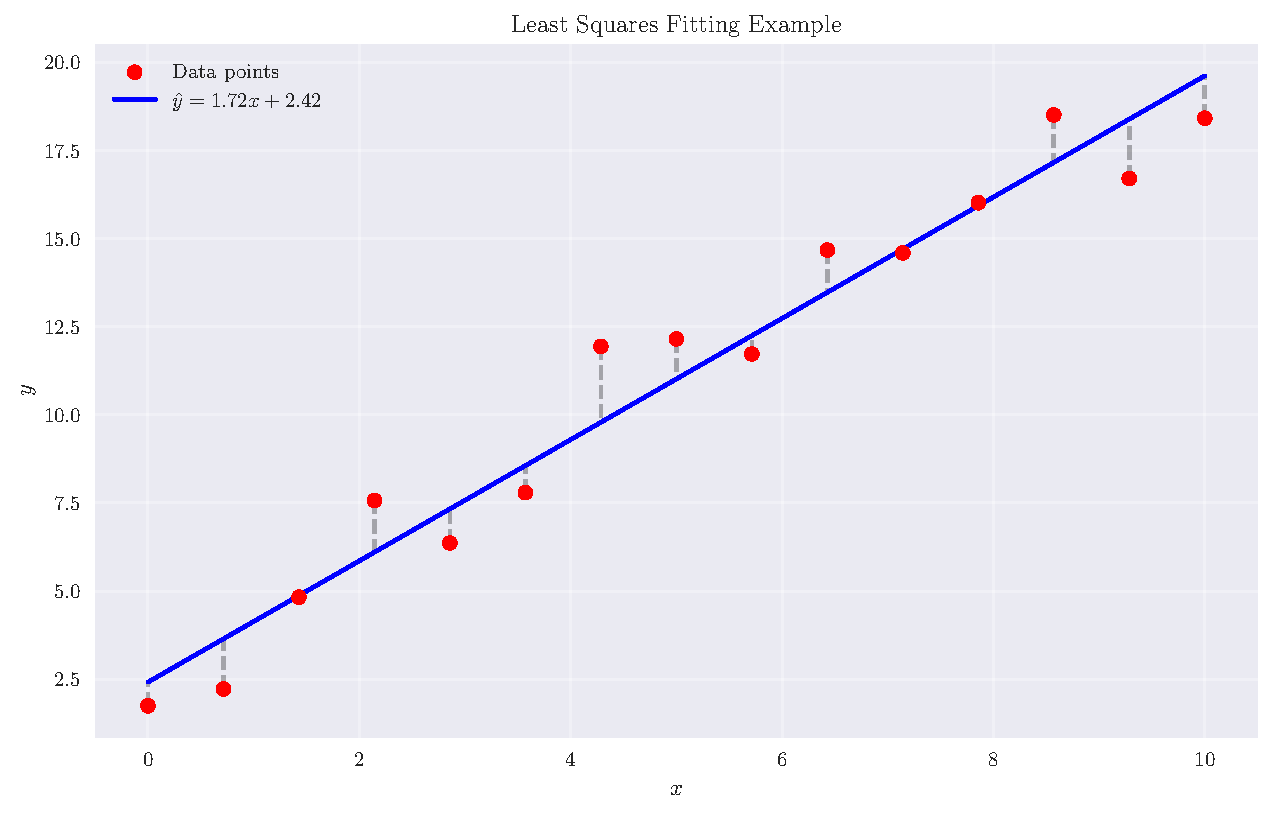
\includegraphics[width=0.9\textwidth]{least_squares.pdf}
    \end{center}
    \begin{itemize}
        \item Red points: Observed data with noise
        \item Blue line: Fitted linear model
        \item Dashed lines: Residuals being minimized
    \end{itemize}
\end{frame}

\begin{frame}[fragile]{Implementation Example: Least Squares Estimation}
\begin{lstlisting}[language=Python]
import numpy as np
from scipy.optimize import minimize

class LeastSquaresEstimator:
    def __init__(self, measurements, measurement_model):
        self.y = measurements        # Measurement vector
        self.h = measurement_model   # Measurement model function
        
    def cost_function(self, theta):
        """Compute sum of squared errors."""
        residuals = self.y - self.h(theta)
        return np.sum(residuals**2)
    
    def estimate(self, theta_init):
        """Find parameters that minimize squared error."""
        result = minimize(self.cost_function, theta_init, 
                        method='Nelder-Mead')
        return result.x  # Return optimal parameters
\end{lstlisting}
\end{frame}

\begin{frame}{Maximum Likelihood Estimation}
    \begin{center}
        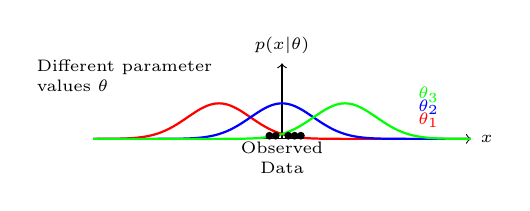
\begin{tikzpicture}[scale=0.8]
            % Draw coordinate axes
            \draw[->] (-3,0) -- (3,0) node[right] {$x$};
            \draw[->] (0,0) -- (0,1.2) node[above] {$p(x|\theta)$};
            
            % Draw three Gaussian curves with different means
            \draw[thick,red,domain=-3:3,samples=100] 
                plot (\x,{exp(-(\x+1)^2/0.5)/sqrt(2*pi*0.5)}) 
                node[right] at (2,0.3) {$\theta_1$};
            \draw[thick,blue,domain=-3:3,samples=100] 
                plot (\x,{exp(-(\x)^2/0.5)/sqrt(2*pi*0.5)}) 
                node[right] at (2,0.5) {$\theta_2$};
            \draw[thick,green,domain=-3:3,samples=100] 
                plot (\x,{exp(-(\x-1)^2/0.5)/sqrt(2*pi*0.5)}) 
                node[right] at (2,0.7) {$\theta_3$};
            
            % Draw data points
            \foreach \x in {-0.2,0.1,0.3,-0.1,0.2}
                \node[circle,fill=black,inner sep=1pt] at (\x,0.05) {};
                
            % Add annotations
            \node[align=center] at (0,-0.3) {Observed\\Data};
            \node[align=left] at (-2.5,1) {Different parameter\\values $\theta$};
        \end{tikzpicture}
    \end{center}
    \vspace{-0.5cm}
    \begin{itemize}
        \item Find parameters $\theta$ that maximize the likelihood of observed data
        \item $\theta_{MLE} = \argmax_\theta \prod_{i=1}^n p(x_i|\theta)$
        \item Blue curve ($\theta_2$) shows the maximum likelihood estimate
    \end{itemize}
\end{frame}

\begin{frame}[fragile]{Implementation Example: Maximum Likelihood Estimation}
\begin{lstlisting}[language=Python]
import numpy as np
from scipy.stats import norm
from scipy.optimize import minimize

class MLEstimator:
    def __init__(self, measurements, measurement_model):
        self.y = measurements        # Measurement vector
        self.h = measurement_model   # Measurement model function
        
    def neg_log_likelihood(self, theta):
        """Compute negative log-likelihood."""
        residuals = self.y - self.h(theta)  # Assuming Gaussian noise model
        return -np.sum(norm.logpdf(residuals))
    
    def estimate(self, theta_init):
        """Find parameters that maximize likelihood."""
        result = minimize(self.neg_log_likelihood, theta_init, 
                        method='Nelder-Mead')
        return result.x  # Return optimal parameters
\end{lstlisting}
\end{frame}

\begin{frame}{Sensor Fusion Overview}
    \begin{center}
        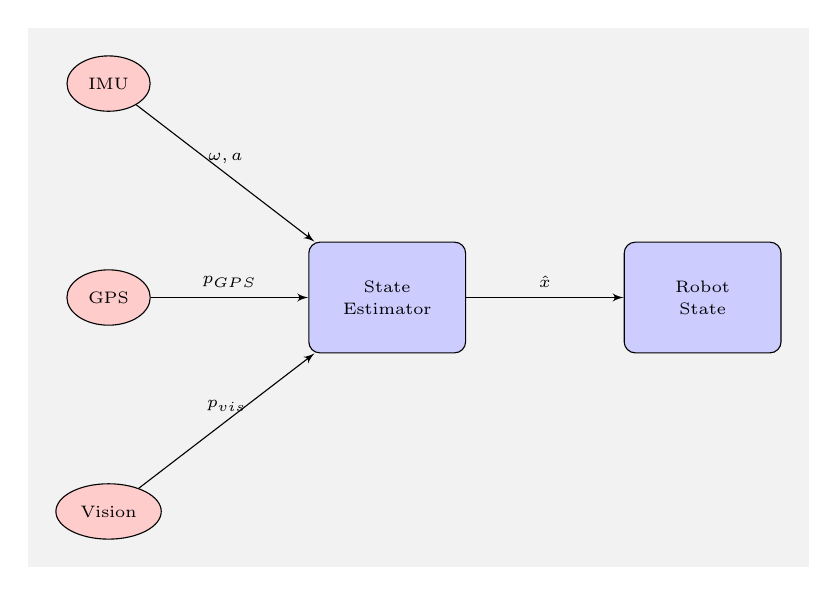
\begin{tikzpicture}[node distance=2cm,auto]
            % Sensors
            \node [cloud] (imu) {IMU};
            \node [cloud] (gps) [below=of imu] {GPS};
            \node [cloud] (vision) [below=of gps] {Vision};
            
            % Fusion block
            \node [block] (fusion) [right=of gps] {State\\Estimator};
            
            % Output
            \node [block] (state) [right=of fusion] {Robot\\State};
            
            % Connect everything
            \path [line] (imu) -- node[above] {$\omega, a$} (fusion);
            \path [line] (gps) -- node[above] {$p_{GPS}$} (fusion);
            \path [line] (vision) -- node[above] {$p_{vis}$} (fusion);
            \path [line] (fusion) -- node[above] {$\hat{x}$} (state);
            
            % Background
            \begin{scope}[on background layer]
                \node[rectangle, fill=gray!10, fit=(imu) (vision) (state),
                      inner sep=1em] {};
            \end{scope}
        \end{tikzpicture}
    \end{center}
\end{frame}

\section{Linear Dynamical Systems}

\begin{frame}{State-Space Models}
    \begin{itemize}
        \item<1-> \textbf{System Dynamics:}
            \begin{align*}
                x_{k+1} &= Ax_k + Bu_k + w_k \\
                y_k &= Cx_k + v_k
            \end{align*}
        \item<2-> \textbf{Components:}
            \begin{itemize}
                \item State vector $x_k$
                \item Input vector $u_k$
                \item Measurement vector $y_k$
                \item Process noise $w_k$
                \item Measurement noise $v_k$
            \end{itemize}
    \end{itemize}
\end{frame}

\begin{frame}{Case Study: Mars Rover Navigation}
    \begin{itemize}
        \item<1-> \textbf{State Variables:}
            \begin{itemize}
                \item Position (x, y, z)
                \item Orientation (roll, pitch, yaw)
                \item Velocities
            \end{itemize}
        \item<2-> \textbf{Sensors:}
            \begin{itemize}
                \item Visual odometry
                \item Inertial measurement unit (IMU)
                \item Sun sensors
            \end{itemize}
        \item<3-> \textbf{Challenges:}
            \begin{itemize}
                \item Wheel slippage
                \item Varying terrain
                \item Limited computational resources
            \end{itemize}
    \end{itemize}
\end{frame}

\begin{frame}[fragile]{Implementation Example: State-Space Model}
\begin{lstlisting}[language=Python]
import numpy as np
from scipy.stats import multivariate_normal

class LinearStateSpaceModel:
    def __init__(self, A, B, C, Q, R):
        self.A = A  # State transition matrix
        self.B = B  # Input matrix
        self.C = C  # Measurement matrix
        self.Q = Q  # Process noise covariance
        self.R = R  # Measurement noise covariance
        
    def propagate_state(self, x, u=None):
        """Propagate state forward one step."""
        w = multivariate_normal.rvs(mean=np.zeros(x.shape), cov=self.Q)
        if u is not None:
            return self.A @ x + self.B @ u + w
        return self.A @ x + w
    
    def get_measurement(self, x):
        """Get noisy measurement of current state."""
        v = multivariate_normal.rvs(mean=np.zeros(self.C.shape[0]), cov=self.R)
        return self.C @ x + v
\end{lstlisting}
\end{frame}

\begin{frame}{State-Space Model}
    \begin{center}
        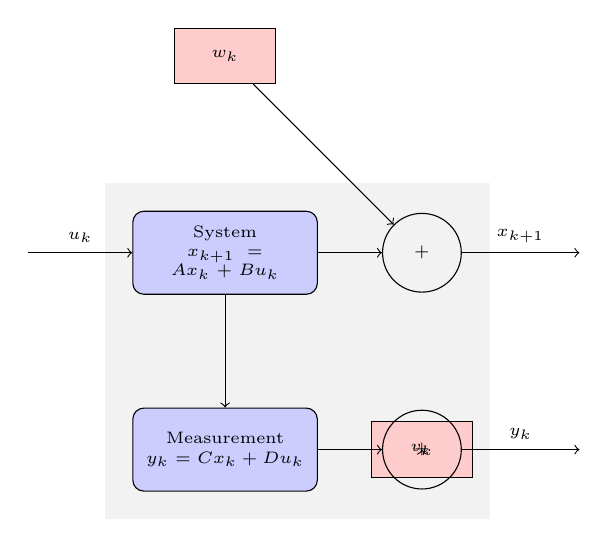
\begin{tikzpicture}[node distance=2.5cm,auto]
            % Define block styles
            \tikzstyle{block} = [rectangle, draw, fill=blue!20, 
                text width=6em, text centered, rounded corners, minimum height=3em]
            \tikzstyle{sum} = [circle, draw, inner sep=0pt,minimum size=1cm]
            \tikzstyle{input} = [coordinate]
            \tikzstyle{output} = [coordinate]
            \tikzstyle{noise} = [rectangle, draw, fill=red!20, 
                text width=3em, text centered, minimum height=2em]
            
            % Place nodes
            \node [input] (input) {};
            \node [block, right of=input] (system) {System\\$x_{k+1} = Ax_k + Bu_k$};
            \node [block, below of=system] (measurement) {Measurement\\$y_k = Cx_k + Du_k$};
            \node [noise, above of=system] (process) {$w_k$};
            \node [noise, right of=measurement] (sensor) {$v_k$};
            \node [sum, right of=system] (sum1) {$+$};
            \node [sum, right of=measurement] (sum2) {$+$};
            
            % Connect nodes
            \draw [->] (input) -- node {$u_k$} (system);
            \draw [->] (system) -- (sum1);
            \draw [->] (sum1) -- node {$x_{k+1}$} ++(2,0);
            \draw [->] (process) -- (sum1);
            \draw [->] (system) -- (measurement);
            \draw [->] (measurement) -- (sum2);
            \draw [->] (sensor) -- (sum2);
            \draw [->] (sum2) -- node[name=y] {$y_k$} ++(2,0);
            
            % Add background
            \begin{scope}[on background layer]
                \node[rectangle, fill=gray!10, fit=(system) (measurement) (sum1) (sum2),
                      inner sep=1em] {};
            \end{scope}
        \end{tikzpicture}
    \end{center}
    \vspace{-0.5cm}
    \begin{itemize}
        \item State equation models system dynamics
        \item Measurement equation relates states to observations
        \item Process noise $w_k$ and measurement noise $v_k$ capture uncertainties
    \end{itemize}
\end{frame}

\section{Next Steps}

\begin{frame}{Preparation for Next Lecture}
    \begin{itemize}
        \item<1-> \textbf{Review:}
            \begin{itemize}
                \item Matrix operations
                \item Probability concepts
                \item Basic Python programming
            \end{itemize}
        \item<2-> \textbf{Setup:}
            \begin{itemize}
                \item Install Linux if needed
                \item Configure ROS2 environment
                \item Test Python scientific libraries
            \end{itemize}
        \item<3-> \textbf{Reading:}
            \begin{itemize}
                \item Skim Kalman filter basics
                \item Review assigned papers
                \item Explore interactive tutorials
            \end{itemize}
    \end{itemize}
\end{frame}

\begin{frame}{Questions?}
    \begin{center}
        \Huge Thank you!
        
        \vspace{1cm}
        \normalsize
        Contact: jdas5@asu.edu
    \end{center}
\end{frame}

\begin{frame}{Course Assessment: Quiz Components}
\begin{itemize}
    \item \textbf{Part 1: Robotics and AI Fundamentals}
    \begin{itemize}
        \item Tests foundational knowledge in robotics and AI
        \item Key topics: SLAM, LiDAR, occupancy grids, GPS challenges, path planning
        \item Required score: 60\% to proceed to Part 2
    \end{itemize}
    \item \textbf{Part 2: Advanced Concepts}
    \begin{itemize}
        \item Tests understanding of tutorial concepts
        \item Topics covered:
        \begin{itemize}
            \item Multi-view geometry and stereo vision
            \item SLAM systems and loop closure
            \item Kalman filter parameters and tuning
            \item Sampling strategies for exploration
            \item Error analysis in rock mapping
        \end{itemize}
    \end{itemize}
\end{itemize}
\end{frame}

\begin{frame}{Quiz Topics and Course Content}
\begin{itemize}
    \item \textbf{Foundational Topics (Part 1)}
    \begin{itemize}
        \item SLAM and LiDAR: Core to robot perception and mapping
        \item Occupancy grids: Probabilistic environment representation
        \item GPS challenges: Motivation for robust state estimation
        \item Path planning: Essential for autonomous navigation
    \end{itemize}
    \item \textbf{Advanced Applications (Part 2)}
    \begin{itemize}
        \item Stereo vision: Depth estimation for rock mapping
        \item Loop closure: Improving map consistency
        \item Kalman filters: State estimation for robot localization
        \item Sampling strategies: Efficient exploration algorithms
        \item Error analysis: Ensuring reliable measurements
    \end{itemize}
\end{itemize}
\end{frame}

\begin{frame}{Least Squares Visualization}
    \begin{center}
        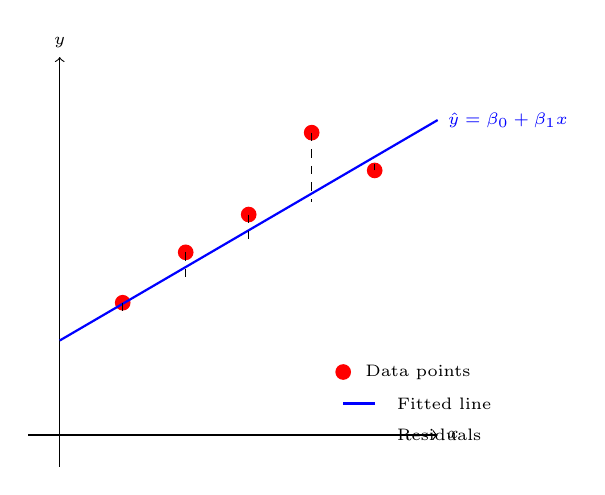
\begin{tikzpicture}[scale=0.8]
            % Draw coordinate axes
            \draw[->] (-0.5,0) -- (6,0) node[right] {$x$};
            \draw[->] (0,-0.5) -- (0,6) node[above] {$y$};
            
            % Draw data points
            \node[circle,fill=red,inner sep=2pt] at (1,2.1) {};
            \node[circle,fill=red,inner sep=2pt] at (2,2.9) {};
            \node[circle,fill=red,inner sep=2pt] at (3,3.5) {};
            \node[circle,fill=red,inner sep=2pt] at (4,4.8) {};
            \node[circle,fill=red,inner sep=2pt] at (5,4.2) {};
            
            % Draw the fitted line
            \draw[thick,blue] (0,1.5) -- (6,5) node[right] {$\hat{y} = \beta_0 + \beta_1x$};
            
            % Draw error bars
            \draw[dashed] (1,2.1) -- (1,1.9);
            \draw[dashed] (2,2.9) -- (2,2.5);
            \draw[dashed] (3,3.5) -- (3,3.1);
            \draw[dashed] (4,4.8) -- (4,3.7);
            \draw[dashed] (5,4.2) -- (5,4.3);
            
            % Add legend
            \node[circle,fill=red,inner sep=2pt] at (4.5,1) {};
            \node[right] at (4.7,1) {Data points};
            \draw[thick,blue] (4.5,0.5) -- (5,0.5);
            \node[right] at (5.2,0.5) {Fitted line};
            \draw[dashed] (4.5,0) -- (5,0);
            \node[right] at (5.2,0) {Residuals};
        \end{tikzpicture}
    \end{center}
    \vspace{-0.5cm}
    \begin{itemize}
        \item Minimize sum of squared residuals: $\min_{\beta_0,\beta_1} \sum_{i=1}^n (y_i - (\beta_0 + \beta_1x_i))^2$
        \item Residuals shown as dashed lines between data points and fitted line
    \end{itemize}
\end{frame}

\begin{frame}{Mars Rover Navigation Example}
    \begin{center}
        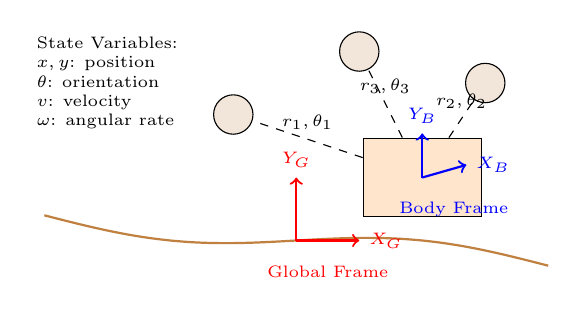
\begin{tikzpicture}[scale=0.8]
            % Define styles for coordinate frames
            \tikzstyle{frame} = [thick, ->]
            \tikzstyle{rover} = [rectangle, draw, fill=orange!20, 
                minimum width=1.5cm, minimum height=1cm]
            \tikzstyle{landmark} = [circle, draw, fill=brown!20,
                minimum size=0.5cm]
            
            % Draw Mars surface (curved line)
            \draw[thick,brown,domain=-4:4,smooth] 
                plot (\x,{0.2*sin(\x*45) - 0.1*\x});
            
            % Draw global frame
            \draw[frame,red] (0,0) -- (1,0) node[right] {$X_G$};
            \draw[frame,red] (0,0) -- (0,1) node[above] {$Y_G$};
            \node[red] at (0.5,-0.5) {Global Frame};
            
            % Draw rover and its body frame
            \node[rover] (rover) at (2,1) {};
            \draw[frame,blue] (2,1) -- (2.7,1.2) node[right] {$X_B$};
            \draw[frame,blue] (2,1) -- (2,1.7) node[above] {$Y_B$};
            \node[blue] at (2.5,0.5) {Body Frame};
            
            % Draw landmarks
            \node[landmark] (l1) at (-1,2) {};
            \node[landmark] (l2) at (3,2.5) {};
            \node[landmark] (l3) at (1,3) {};
            
            % Draw measurements
            \draw[dashed] (rover) -- (l1) node[midway,above] {$r_1,\theta_1$};
            \draw[dashed] (rover) -- (l2) node[midway,above] {$r_2,\theta_2$};
            \draw[dashed] (rover) -- (l3) node[midway,above] {$r_3,\theta_3$};
            
            % Add state variables
            \node[align=left] at (-3,2.5) {State Variables:\\
                $x, y$: position\\
                $\theta$: orientation\\
                $v$: velocity\\
                $\omega$: angular rate};
        \end{tikzpicture}
    \end{center}
    \vspace{-0.5cm}
    \begin{itemize}
        \item Rover state estimated using multiple coordinate frames
        \item Landmarks provide relative measurements $(r_i,\theta_i)$
        \item Global frame used for absolute positioning
    \end{itemize}
\end{frame}

\end{document} 